\documentclass[a4paper]{article}
\usepackage{natbib}
\usepackage{url}
\usepackage{hyperref}
\hypersetup{
    colorlinks,
    citecolor=black,
    filecolor=black,
    linkcolor=black,
    urlcolor=black,
	linktoc=all,
	bookmarksdepth=paragraph
}
\usepackage[cyr]{aeguill}
\usepackage[utf8]{inputenc}
\usepackage[francais]{babel}
\usepackage{amsmath}
\usepackage{graphicx}
\usepackage{parskip}
\usepackage{fancyhdr}
\usepackage{listings}

%%configuration de listings
\lstset{
	language=PHP,
	basicstyle=\ttfamily\footnotesize, %
	identifierstyle=\color{red}, %
	keywordstyle=\bfseries\color{blue}, %
	stringstyle=\color{black!60}, %
	commentstyle=\color{green!95!yellow!1}, %
	columns=flexible, %
	tabsize=2, %
	extendedchars=true, %
	showspaces=false, %
	showstringspaces=false, %
	numbers=left, %
	numberstyle=\tiny, %
	breaklines=true, %
	breakautoindent=true, %
	captionpos=b
}

\title{Réalisation d'un site de partage et de création de dessins}
\author{Lucien Aubert $\newline$ Tom Henoch}

\makeatletter
\let\theauthor\@author
\let\thetitle\@title
\makeatother

\pagestyle{fancy}
\fancyhf{}
\chead{\thetitle}
\cfoot{\raggedleft\thepage}
\begin{document}

\begin{titlepage}
	\centering
    \vspace*{0.5 cm}
    \href{http://iut.univ-amu.fr/sites/arles}{
\includegraphics[scale = 0.15]{logo-amu.png}}\\[1.0 cm]
    \textsc{\LARGE Aix-Marseille Université}\\[2.0 cm]
	\textsc{\Large M3103 - Programmation Web côté serveur}\\[0.5 cm]
	\rule{\linewidth}{0.2 mm} \\[0.4 cm]
	{ \huge \bfseries \thetitle}\\
	\rule{\linewidth}{0.2 mm} \\[1.5 cm]

	\begin{minipage}[t]{0.4\textwidth}
		\begin{flushleft} \large
			\emph{Auteurs :}\\
			\theauthor
			\end{flushleft}
			\end{minipage}~
			\begin{minipage}[t]{0.4\textwidth}
			\begin{flushright} \large
			\begin{flushleft}
			\emph{Enseignants :} \\
			Brett Desbenoit $\newline$Laurent Carmignac
		 \end{flushleft}
		\end{flushright}
	\end{minipage}\\[2 cm]

	\vfill
\end{titlepage}
\pagestyle{empty}
\tableofcontents
\pagebreak
\pagestyle{fancy}
\setcounter{page}{1}
\section{Introduction}
L'utilisateur sera en mesure de dessiner avec des outils basiques (crayon, carré, cercle, lettrages) et de partager sa création. Les dessins ainsi créés sont modifiables par plusieurs utilisateurs.

Les utilisateurs pourront commenter les dessins et les marquer comme "J'aime".

\section{Structure}
L'application est composée de trois modules qui interagissent :
\begin{itemize}
	\item un serveur web (site + base de données)
	\item un serveur spécifique à l'édition de dessin
	\item une application client servie par le serveur web
\end{itemize}

\begin{center}
	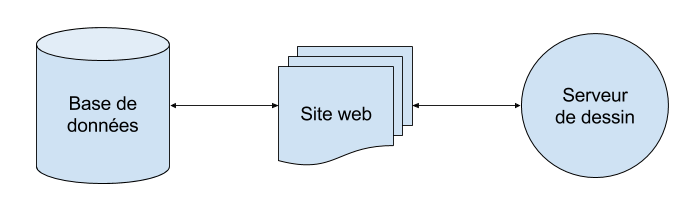
\includegraphics[width=0.8\textwidth]{sketcher_global_structure.png}
\end{center}

La base de données n'est accessible que par le site web, doté d'une API type REST permettant au serveur de dessin de lui passer des requêtes.

\subsection{Serveur Web}
Le site web est développé avec le framework Symfony 3 et utilise une base de données MariaDB. Il est hébergé sur un serveur Apache 2.4.

Il joue les rôles d'interface utilisateur et de gestionnaire de base de données.

C'est lui qui donne la permission au serveur de dessin de démarrer une connexion avec un client.

Pour l'utilisateur, il permet de
\begin{itemize}
	\item s'inscrire
	\item se connecter (authentification par nom et mot de passe)
	\item créer un nouveau dessin
	\item consulter la galerie
	\item rechercher un dessin par nom
	\item rechercher un dessin par tag
	\item modifier son profil
	\item modifier ses dessins (titre, auteurs, tags)
\end{itemize}

\subsubsection{Ajax}

Nous avons privilégié des interfaces avancées pour certains formulaires (champs d'édition de tags, d'auteurs, de titre). Pour se faire nous avons eu recours à l'utilisation de \texttt{XMLHttpRequest}, une object Javascript qui permet de faire envoyer des requêtes HTTP par le client. Le client envoie donc des requêtes \texttt{GET} vers le serveur pour signaler l'ajout ou la suppression d'un tag ou d'un auteur, le serveur envoie sa réponse sous forme d'un fichier JSON avec une message d'erreur ou de succès qui sera parsé par le client pour afficher une notification.

\subsubsection{Plan du site}
\begin{center}
	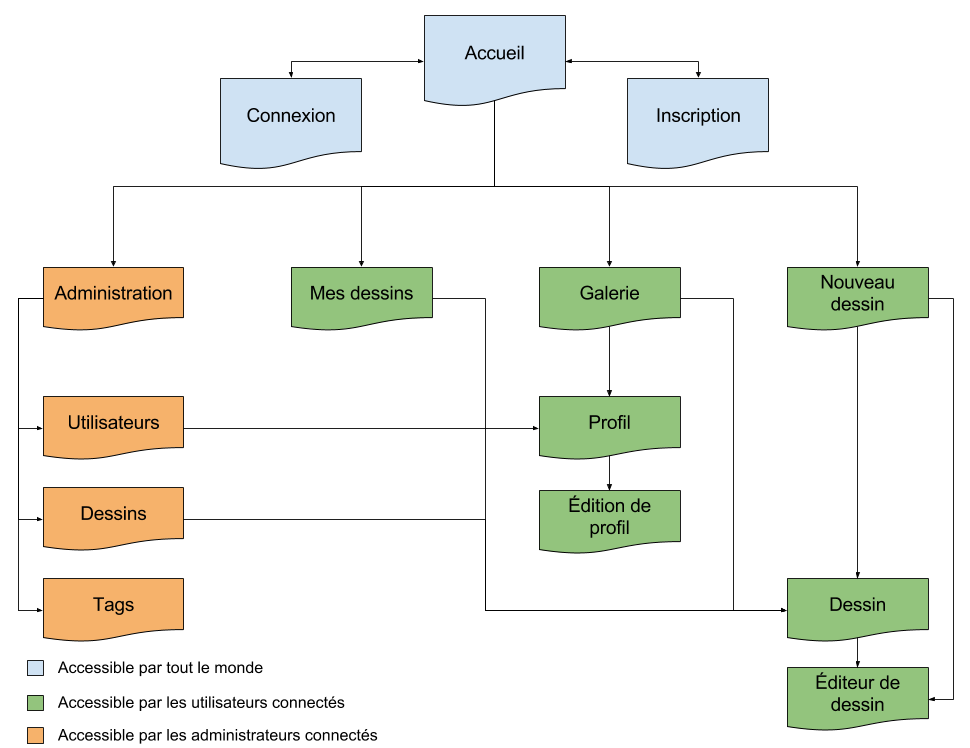
\includegraphics[width=1\textwidth]{sketcher_sitemap.png}
\end{center}

Les pages protégées rediriges vers la page de connexion si l'utilisateur n'est pas connecté et vers la page d'accueil quand il tente d'accéder à du contenu qui ne lui est pas accessible.

Symfony aidant, il nous est possible de vérifier si l'utilisateur nous a donné le cookie d'une session grâce à cette simple condition, \texttt{\$this} étant notre controleur.
\begin{lstlisting}
if(!$this->getUser())
	return $this->redirectToRoute('login');
\end{lstlisting}

La chaîne \texttt{'login'} correspond ici à la route vers laquelle rediriger le client. Le système de routing du framework permet de définir des routes en leur attribuant un nom, des arguments et une méthode qui sera exécutée quand la route sera demandée par un client. Ces définitions sont faites sous forme de commentaires formatés comme suit.
\begin{lstlisting}
	/**
	* @Route(
	*   "/sketch/{sketchId}",
	*   requirements={"sketchId": "\d+"},
	*   name="sketch"
	* )
	*/
\end{lstlisting}
Les fichiers source sont ensuite traités par Symfony et les commentaires parsés pour produire un module de routage sur mesure.

\section{Conclusion}
La création de cette application nous a permis de découvrir le framework Symfony 3 ainsi que la technologie des WebSockets. L'utilisation du Javascript pour le développement complet de l'outil de dessin nous a appris beaucoup sur ce langage, tant côté serveur que côté client.

Le déploiement de l'application a été un défi que nous avons relevé en nous documentant sur le serveur web que nous utilisions, Apache 2.4, ce qui nous a permis d'approfondir les connaissances que nous avons acquis en cours de réseau.
\newpage
\bibliographystyle{unsrt}
\bibliography{biblio}

\end{document}
